\documentclass[11pt]{beamer}
\usetheme{Boadilla}
\usepackage[latin2]{inputenc}
\usepackage[english]{babel}
\usepackage{amsmath}
\usepackage{amsfonts}
\usepackage{amssymb}
\usepackage{graphicx}
\author{Aryaman Sharma}
\title{COMP3702 Tutorial 4}
%\setbeamercovered{transparent} 
%\setbeamertemplate{navigation symbols}{} 
%\logo{} 
%\institute{} 
\date{August 2022} 
%\subject{} 
\begin{document}

\begin{frame}
	\titlepage
\end{frame}


\begin{frame}{Constraint Satisfaction Problem (CSP)}
\begin{definition}[Costraint Satisfaction Problem]
A CSP is given by:
\begin{itemize}
	\pause
	\item A set of variable $V_1, V_2, ..., V_n$.\pause
	\item Each variable $V_i$ has an associated domain of possible values. \pause
	\item A set of constraints on various subsets of the variables which are logical predicates specifying legal combinations of values for these variables. \pause
	\item A \textbf{Model} of a CSP is an assignment of values variables that satisfies all of the constraints. 
\end{itemize}
\end{definition}
\end{frame}

\begin{frame}{4.1}
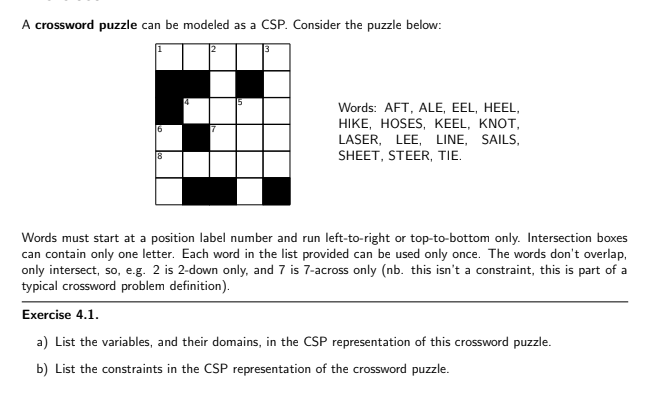
\includegraphics[scale=0.5]{images/41.png}
\end{frame}

\begin{frame}{4.1 a}
\textbf{Variables} \pause
\begin{itemize}
	\item 1-across \pause
	\item 2-down, 3-down, 4-across, 5-down, 6-down, 7-across and 8-across.
\end{itemize}
\pause
\textbf{Domains} \pause
\begin{itemize}
	\item For all variables: $\{$AFT, ALE, ..., TIE $\}$
\end{itemize}
\end{frame}

\begin{frame}{4.1 b}
List \textbf{constraints} in this CSP \pause
\begin{itemize}
	\item \textbf{Domain constraint} Variable can only be set to words of correct length.
	\pause
	\item \textbf{Binary constraint} Letters used at intersection must be equal.\pause
	\item \textbf{Global constraint} Each word is used only once.
\end{itemize}
\end{frame}

\begin{frame}{Constraint graph: A bipartite graph}
\pause
\begin{itemize}
	\item There is a circle or oval-shaped node for each variable.
	\pause
	\item There is a rectangular node for each constraint.\pause
	\item There is a domain of values associated with each variable node.\pause
	\item There is an arc from variable X to each constraint that involves X.\pause
\end{itemize}
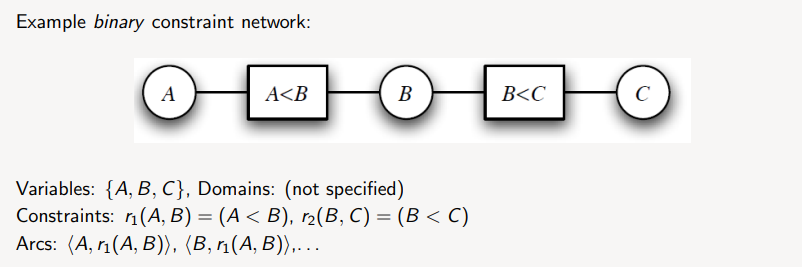
\includegraphics[scale=0.4]{images/graphexample.png}
\end{frame}

\begin{frame}{4.2}
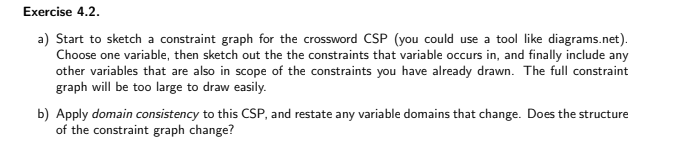
\includegraphics[scale=0.5]{images/42.png}
\end{frame}

\begin{frame}{4.2 a}
\pause
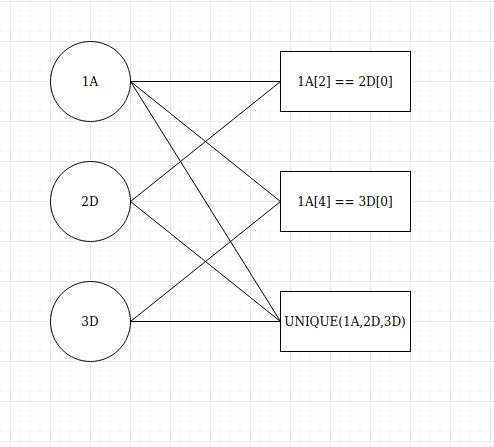
\includegraphics[scale=0.5]{images/42graph.png}
\end{frame}

\begin{frame}{Domain consistency}
\pause
\begin{itemize}
	\item Prune the domains as much as possible before selecting values from them.\pause
	\item A variable is \textbf{Domain consistent} if no value if the domain of the node is ruled impossible by any on the constraints.\pause
\end{itemize}
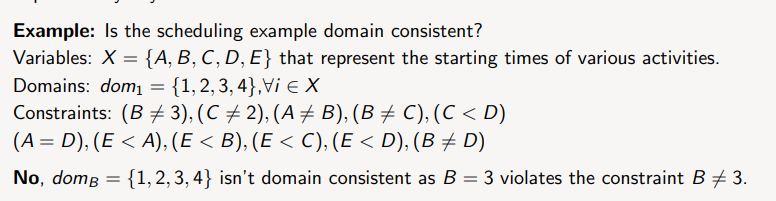
\includegraphics[scale=0.4]{images/dcexample.png}
\end{frame}

\begin{frame}{4.2 b}
\textbf{Apply domain consistency to this CSP, and restate any variable domains that change. Does the structure of the constraint graph change?}\pause
\begin{itemize}
	\item Domains are reduced to those with answers with word lengths that are consistent with the number of blank spaces, so all variable domains are changed.\pause
	\item Updated domains: \pause
	\begin{itemize}
		\item $dom[1A]=\{HOSES, LASER, SAILS, SHEET, STEER\}$\pause
		\item $dom[2D] = \{HOSES, LASER, SAILS, SHEET, STEER\}$
		\item $dom[3D] = \{HOSES, LASER, SAILS, SHEET, STEER\}$
		\item $dom[4A] = \{HEEL, HIKE, KEEL, KNOT, LINE\}$
		\item $dom[5D] = \{HEEL, HIKE, KEEL, KNOT, LINE\}$
		\item $dom[6D] = \{AFT,ALE,EEL,LEE,TIE\}$
		\item $dom[7A] = \{AFT,ALE,EEL,LEE,TIE\}$
		\item $dom[8A] = \{HOSES, LASER, SAILS, SHEET, STEER\}$
	\end{itemize}\pause
	\item \textbf{Does the structure of the graph change?}
\end{itemize}
\end{frame}

\begin{frame}{Backtracking search}
\pause
\begin{itemize}
	\item Systematically explore domain by instantiating the variables one at a time. \pause
	\item Evaluate each constraint predicate as soon as all its variables are bound.\pause
	\item Any partial assignment that dosen't satisfy the constraint can be pruned. \pause
	\item Essentially we "brute force" our way to a solution.
\end{itemize}
\end{frame}

\begin{frame}{Sudoku backtracking example}
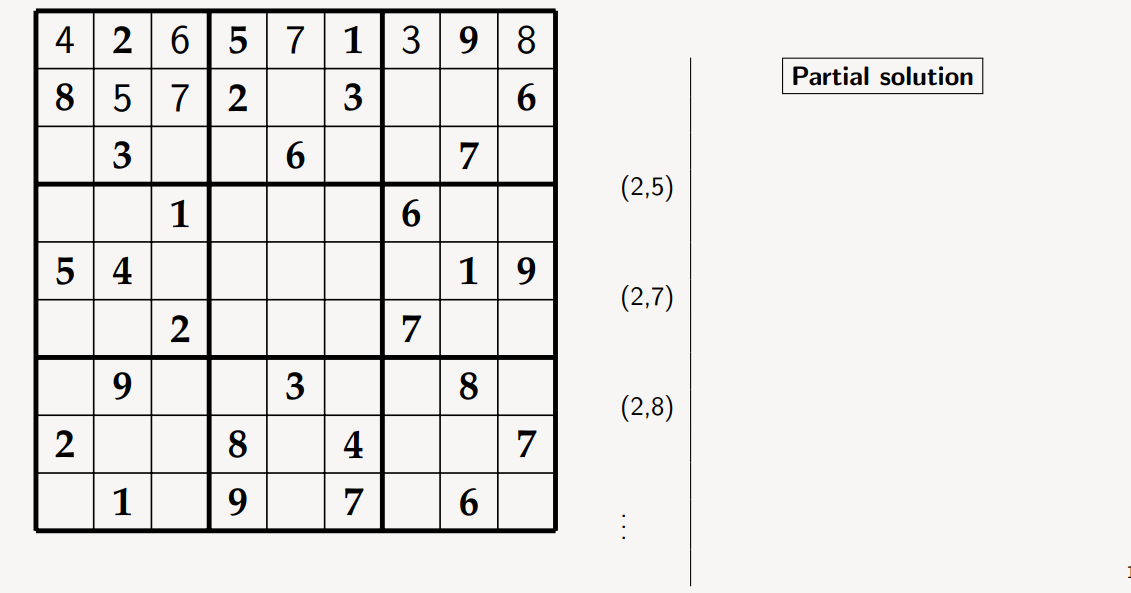
\includegraphics[scale=0.3]{images/sudoku.png}
\end{frame}

\begin{frame}{4.3}
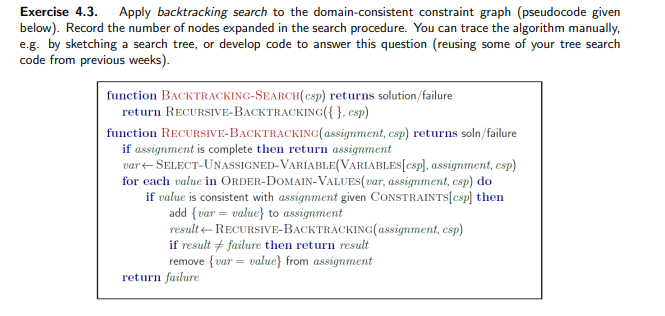
\includegraphics[scale=0.5]{images/43.png}
\end{frame}

\begin{frame}{4.3}
\pause
\begin{itemize}
	\item Select 1A, as the first unassigned variable. \pause
	\item Check if the first value in domain of 1-across conflicts with the existing (empty) assignment; it dosen't, so expand 1A$=HOSES$.\pause
	\item Now select 2-down, as the next unassigned variable; this is using the recursive function call. \pause
	\item Check if the first value in domain of 2D, HOSES, conflicts with the existing assignment. It does! $\implies$ throw it away.\pause
	\item ... so on \pause
\end{itemize}
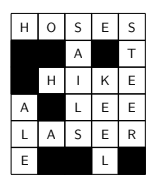
\includegraphics[scale=0.4]{images/34solved.png}
\end{frame}

\begin{frame}{Arc-consistency}
\begin{definition}[Arc consistency]
An arc $<X, r(X,\bar{Y})>$ is arc consistent if, for each value $x\in dom(X)$, there is some value $\bar{y}\in Dom(\bar{Y})$ such that $r(x,\bar{y})$ is satisfied. A network is arc consistent if all arcs are arc consistent.
\end{definition}
\pause
\begin{itemize}
	\item Here $r(X,\bar{Y})$ is a constraint.
\end{itemize}
\pause
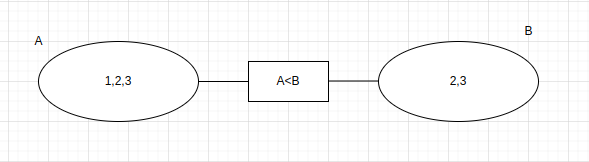
\includegraphics[scale=0.3]{images/699.png}
\end{frame}

\begin{frame}{4.4}
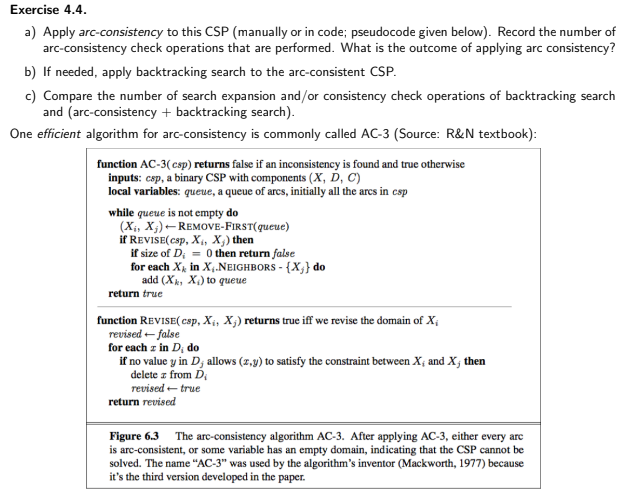
\includegraphics[scale=0.4]{images/44.png}
\end{frame}

\begin{frame}{4.4}
\begin{itemize}
	\item 1A = $\{$HOSES,LASER,SAILS,SHEET,STEER$\}$ pause
	\item Check for a value in the domain of 2D consistent with each element in 1A. \\
	2D = $\{$HOSES,LASER,SAILS,SHEET,STEER$\}$\pause
	\item Remove SAILS, SHEET, STEER from 1A.\\
	1A = $\{$HOSES,LASER$\}$ \pause
	\item Check for a value in the domain of 3D consistent with each element in 1A.\\
	3D = $\{$HOSES,LASER,SAILS,SHEET,STEER$\}$\pause
	\item Remove LASER from 1A
	\item This implies that 1A must be HOSES, as all other values are not arc consistent.
	\item Now move onto next variable...
\end{itemize}
\end{frame}

\begin{frame}{Code}
https://gist.github.com/aryaman-sh/8f73ae3196c589f5b5bf6a1bf4c0a37e
\\

\includegraphics[scale=0.4]{code.png}
\end{frame}

\begin{frame}{2021 exam question}
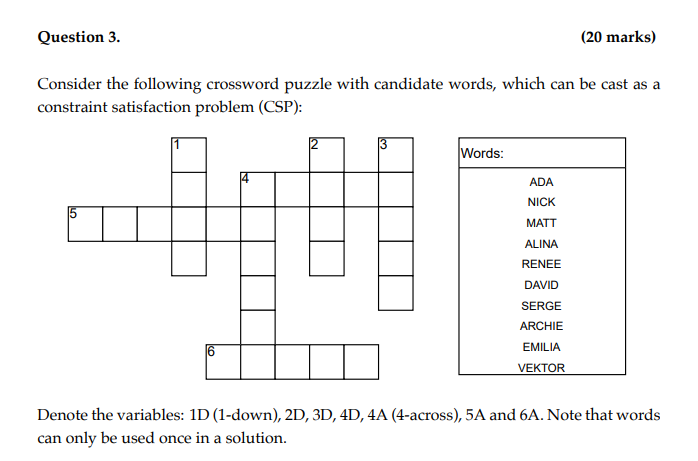
\includegraphics[scale=0.3]{images/2021.png}
\begin{itemize}
	\item List all binary constraints.
	\item Apply domain consistency.
	\item Apply arc consistency.
	\item Apply backtracking to domain consistent CSP use ordering (1D,2D,3D,4D,4A,5A,6A)
\end{itemize}
\end{frame}
\end{document}